\documentclass[conference]{IEEEtran}

\usepackage[utf8]{inputenc}
\usepackage[T1]{fontenc}
\usepackage[brazilian]{babel}
\usepackage{amsmath}
\usepackage{amssymb}
\usepackage{graphicx}
\usepackage{booktabs}
\usepackage{float}
\usepackage{hyperref}
\hypersetup{
    colorlinks=true,
    linkcolor=black,
    citecolor=black,
    urlcolor=blue,
}

\graphicspath{{../figures/}{./}}

\title{
    {\huge Trabalho 2 - Implementação de Algoritmos Distribuídos} \\[0.2cm]
    {\small MC714 - Sistemas Distribuídos - Unicamp}
}

\author{\IEEEauthorblockN{Celso Gabriel Ferreira Marçal Prado (RA: 235393)}
\IEEEauthorblockA{\texttt{c235393@dac.unicamp.br}}
\and
\IEEEauthorblockN{Giovanni Santos Scalabrin (RA: 281210)}
\IEEEauthorblockA{\texttt{g281210@dac.unicamp.br}}}

\begin{document}

\maketitle

\section*{Resumo}
Sistemas distribuídos exigem mecanismos de coordenação que garantam acesso
exclusivo a recursos compartilhados, efetivação atômica de operações que
envolvem múltiplos nós e observação consistente do estado global. Este
trabalho implementa três algoritmos clássicos integrados em uma aplicação de
liquidação financeira distribuída, o \texttt{distrib-ledger}, na qual cada nó
executa como processo independente, comunicando-se exclusivamente pela rede.
O algoritmo de Ricart-Agrawala com relógios lógicos de Lamport serializa o
acesso à seção crítica com exatamente $2(N-1)$ mensagens por entrada, o
compromisso atômico em duas fases com registro persistente em WAL coordena
transferências entre nós e se recupera da queda abrupta do coordenador, e o
snapshot de Chandy-Lamport audita cortes globais consistentes sob tráfego
ativo. As propriedades de correção foram verificadas por 23 testes
automatizados, incluindo o encerramento abrupto real do processo coordenador
antes e depois da decisão. Os experimentos variam o número de nós
($N \in \{3, 5, 7, 9\}$), o atraso de canal ($\Delta \in \{5, 25, 50\}$ ms) e
a carga de transferências ($\lambda \in \{10, 25, 50\}$ tx/s), com dez
repetições independentes por configuração. As medições confirmaram a troca
exata de $2(N-1)$ mensagens em todas as entradas na seção crítica, a
atomicidade em 90 de 90 execuções do protocolo de commit e a conservação
patrimonial em 60 de 60 snapshots sob tráfego concorrente, com recuperação de
queda concluída em 6 a 9 ms.

\section*{Informações de Entrega}
\textbf{Repositório do trabalho}\\
\url{https://github.com/gsscala/t2-mc714}\\
\textbf{Vídeo de demonstração}\\
\url{https://youtu.be/3dndSmKldBw}


\section{Introdução}
A coordenação entre processos é um dos temas centrais dos sistemas
distribuídos, conforme organizado por van Steen e Tanenbaum \cite{vansteen2023},
e os algoritmos de exclusão mútua, de compromisso atômico e de captura de estado
global resolvem três necessidades que costumam coexistir em aplicações
práticas. Um consórcio financeiro distribuído ilustra bem essa convivência, pois
exige serializar o acesso concorrente às contas, efetivar transferências entre
agências de forma totalmente atômica e auditar o patrimônio total sem
interromper a operação.

Este trabalho implementa o \texttt{distrib-ledger}, um sistema bancário
distribuído no qual cada agência é um processo independente com armazenamento
próprio, conforme o enunciado. Três algoritmos clássicos foram integrados a
esse sistema:

\begin{itemize}
    \item \textbf{Ricart-Agrawala \cite{ricart1981algorithm}:} serializa o
    acesso à seção crítica (SC) pela ordem total definida pelos relógios
    lógicos de Lamport \cite{lamport1978time}, sem coordenador central.
    \item \textbf{Two-Phase Commit (2PC) com Write-Ahead Log (WAL) \cite{gray1978notes}:}
    coordena transferências entre nós com decisão atômica, reserva de saldo e
    recuperação baseada na regra de cancelamento presumido
    (\emph{Presumed Abort}).
    \item \textbf{Chandy-Lamport \cite{chandy1985distributed}:} captura cortes
    globais consistentes durante o tráfego, permitindo a um auditor verificar a
    conservação do montante total.
\end{itemize}

Os três algoritmos operam sobre a mesma aplicação. Cada transferência
coordenada pelo 2PC é protegida pela seção crítica do Ricart-Agrawala, e o
snapshot audita o ledger durante transferências ativas, o que integra os
algoritmos em um fluxo único em vez de módulos isolados. O restante deste
texto descreve o modelo do sistema e as hipóteses adotadas, a arquitetura e o
funcionamento dos algoritmos, as propriedades de correção com suas
justificativas, o delineamento experimental e, por fim, os resultados e a
conclusão.

\section{Modelo do Sistema e Hipóteses}
O modelo adotado declara explicitamente as hipóteses sob as quais os
algoritmos operam:

\begin{itemize}
    \item \textbf{Modelo temporal:} parcialmente síncrono, sem limites
    conhecidos sobre atrasos de processamento e de transmissão.
    \item \textbf{Canais:} TCP ponto a ponto com enquadramento por prefixo de
    tamanho e serialização JSON. Por construção são confiáveis e FIFO, pois
    cada envio mantém uma trava por destino e as mensagens de uma conexão são
    processadas em ordem estrita de chegada. Todo envio possui prazo
    explícito de 2 s.
    \item \textbf{Falhas:} queda e recuperação (\emph{crash-recovery}). O
    processo pode ser encerrado abruptamente a qualquer momento por
    \texttt{os.\_exit} e retorna depois recarregando o estado do WAL. Falhas
    bizantinas são desconsideradas.
    \item \textbf{Relógios e persistência:} não há relógios físicos
    sincronizados; a ordenação causal usa relógios lógicos de Lamport
    \cite{lamport1978time}. Todo voto e toda decisão do 2PC passam pelo WAL com
    \texttt{fsync} antes de qualquer envio.
    \item \textbf{Associação:} estática, com lista fixa de nós configurada no
    início da execução.
\end{itemize}

As injeções de atraso, perda, partição e queda são aplicadas apenas nos
cenários que as estudam, de modo que o modelo base assume canais confiáveis,
e os algoritmos foram projetados para preservar suas propriedades mesmo
quando as injeções estão ativas. Pelo teorema FLP \cite{fischer1985impossibility},
a terminação determinística sob falhas de processo exige suposições adicionais,
e o 2PC as obtém com temporizadores de votação, retransmissão idempotente de
decisões e a regra de \emph{Presumed Abort} \cite{gray1978notes}.

\section{Arquitetura e Algoritmos}
Cada nó lógico é um processo independente, executado como contêiner OCI no
ambiente de referência do Docker Compose e como processo nativo nos
experimentos, sempre por meio do mesmo comando. O processo recebe mensagens
por TCP e as despacha ao módulo correspondente, exclusão mútua, compromisso
atômico ou snapshot, processando-as em ordem estrita de chegada, semântica da
qual o Chandy-Lamport depende. Um plano de controle sobre os mesmos canais
permite a um cliente externo disparar operações, consultar estatísticas e
configurar falhas, e é esse mecanismo que os scripts de experimento e a
demonstração em vídeo utilizam para operar o cluster.

\subsection{Exclusão Mútua de Ricart-Agrawala}
O nó mantém os estados RELEASED, WANTED e HELD e um relógio lógico. Para
entrar na SC ele avança o relógio, difunde $\text{RA\_REQUEST}$ com o par
$(T, id)$ e aguarda as $N-1$ respostas. Ao receber um pedido, responde
imediatamente quando o par recebido tem prioridade menor na ordem total, ou
retém a resposta em uma fila de diferimento em caso contrário. Ao sair da SC,
responde a todos os retidos, o que custa $2(N-1)$ mensagens por entrada em
execução sem perdas \cite{ricart1981algorithm}.

Sob perda de mensagens, o nó nunca entra na SC com respostas pendentes, pois
assumir que um par silencioso caiu violaria a segurança quando ele está
apenas lento. Os pedidos são retransmitidos de forma idempotente a cada
500 ms enquanto faltarem respostas, e as duplicatas são absorvidas pela fila
de diferimento sem criar novas permissões. A contrapartida, declarada como
limitação, é que a queda permanente de um par bloqueia novas entradas na SC.

\subsection{Compromisso Atômico em Duas Fases com WAL}
Na primeira fase o coordenador grava \texttt{START\_2PC} e envia
\texttt{PREPARE} aos participantes. Cada participante valida o saldo
disponível e reserva os fundos da transação antes de votar, grava
\texttt{PREPARED} e responde com seu voto. A reserva impede o gasto duplo,
pois transações concorrentes do mesmo emissor competem pelo mesmo saldo
disponível, e \texttt{PREPARE} duplicado reenvia o voto memorizado em vez de
revalidar contra um saldo alterado.

Com votos unânimes o coordenador grava \texttt{COMMITTED}, aplica as
operações localmente, grava \texttt{APPLIED} e difunde
\texttt{GLOBAL\_COMMIT} com retransmissão até receber os ACKs. Diante de voto
negativo ou de tempo esgotado, grava \texttt{ABORTED}, libera as reservas e
difunde \texttt{GLOBAL\_ABORT}. O registro \texttt{APPLIED} garante que a
aplicação das operações ocorra exatamente uma vez, pois a recuperação que
encontra \texttt{COMMITTED} sem \texttt{APPLIED} reaplica as operações uma
única vez.

Ao reiniciar, o coordenador com \texttt{START\_2PC} sem decisão aplica o
\emph{Presumed Abort} e notifica os participantes, enquanto o coordenador com
\texttt{COMMITTED} reaplica localmente e repropaga a decisão aos
participantes retidos. O participante que reinicia em \texttt{PREPARED}
consulta o coordenador e os pares e adota a resposta obtida, mas nunca aborta
unilateralmente quando ninguém conhece o desfecho, pois o coordenador pode
ter decidido COMMIT antes de cair, e a transação permanece in-doubt para o
próximo ciclo de recuperação. O saldo do processo reiniciado é reconstruído
pela reprodução ordenada do WAL, de modo que o estado comprometido sobrevive
à queda.

\subsection{Snapshot Distribuído de Chandy-Lamport}
O iniciador grava seu estado local e envia \texttt{CL\_MARKER} por todos os
canais de saída. Ao receber o primeiro marcador de um snapshot, o nó grava
seu estado, inicia a gravação das mensagens de aplicação nos demais canais de
entrada e repassa o marcador, e os marcadores seguintes encerram a gravação de
cada canal \cite{chandy1985distributed}. As transferências diretas, com débito
no emissor e crédito no receptor, são as mensagens gravadas em trânsito, e o
auditor soma saldos locais e quantias capturadas para verificar a conservação.

A captura do estado e o envio dos marcadores são passos separados, o que abre
uma janela sutil. Uma transferência emitida logo após a captura poderia furar
a fila de envio e chegar ao destino antes do marcador, sendo aplicada no
saldo capturado do emissor e ainda registrada como em trânsito, com contagem
dupla no corte. Um portão de ordenação por destino fecha essa janela, pois o
emissor de mensagens de aplicação aguarda a saída dos marcadores pendentes
antes de transmitir.

\subsection{Injeção de Falhas e Plano de Controle}
O \texttt{FaultInjector} intercepta todo envio e aplica, por semente
pseudoaleatória registrada, atraso fixo ou com \emph{jitter}, descarte
probabilístico, partição bidirecional entre pares específicos e encerramento
abrupto do processo. Os comandos de controle permitem configurar falhas a
quente em um cluster em execução, o que viabiliza tanto os experimentos
automatizados quanto a demonstração em vídeo, sempre com cenários repetíveis.

\section{Propriedades de Correção}
A primeira propriedade é a exclusão mútua da seção crítica,
\begin{equation}
    \forall t, \quad \left| \{ i \in \{1,\dots,N\} : \text{state}_i(t) = \text{HELD} \} \right| \le 1.
    \label{eq:exclusao}
\end{equation}
A justificativa é a usual do algoritmo de Ricart e Agrawala. Se dois nós
estivessem simultaneamente na SC, ambos teriam respondido ao pedido do outro.
Com a ordem total $(T, id)$ e canais FIFO, porém, o pedido de maior prioridade
é retido pelo nó de menor prioridade até que este saia da SC, o que contradiz
a premissa de ocupação conjunta. A retransmissão preserva o argumento, pois
duplicatas não criam novas permissões, apenas recuperam respostas perdidas.

A segunda propriedade é a atomicidade do 2PC, pela qual todos os nós
operacionais chegam ao mesmo desfecho para cada transação,
\begin{equation}
    \forall P_i, P_j:\ \text{dec}(P_i, tx) = \text{dec}(P_j, tx) \in \{\text{COMMIT}, \text{ABORT}\}.
    \label{eq:atomicidade}
\end{equation}
Um único voto negativo impede a confirmação global, e a decisão é difundida
com retransmissão idempotente até o reconhecimento de todos. O participante
in-doubt nunca decide sozinho, o registro \texttt{APPLIED} garante aplicação
exatamente única e a reprodução ordenada do WAL reconstrói o saldo, o que
elimina tanto a divergência de desfechos quanto a perda de aplicações após
uma queda.

A terceira propriedade é a conservação patrimonial no corte capturado pelo
snapshot,
\begin{equation}
    \sum_{i=1}^{N} \text{balance}_i + \sum_{c \in \text{Canais}} \left( \sum_{m \in c} m.\text{amount} \right) = M_{\text{total}},
    \label{eq:conservacao}
\end{equation}
pois toda transferência ou está integralmente dentro do corte, aplicada nos
dois lados capturados, ou fora dele, ou registrada como em trânsito no canal
de entrada. O portão de ordenação de marcadores elimina a única janela de
contagem dupla, e o auditor valida a igualdade em todos os snapshots.

A suíte de testes reproduz os cenários críticos de cada propriedade, com
contenção e atraso na exclusão mútua, queda real do coordenador antes e
depois da decisão, participante in-doubt com coordenador inalcançável,
transferências concorrentes conflitantes e snapshots sob tráfego com
\emph{jitter}. Um teste adicional executa o sistema completo com nós em
processos separados, cobrindo transferência, snapshot, queda abrupta do
coordenador e reinício com recuperação.

\section{Metodologia Experimental}
Todos os experimentos executam cada nó como processo independente
comunicando-se exclusivamente por TCP, por meio do mesmo comando usado pelos
contêineres do \texttt{compose.yaml}. O ambiente registrou Intel Core
i7-1355U com 12 núcleos, Linux 6.8.0 em x86\_64, Python 3.12.3, Docker 29.9.1
e Compose 5.6.0. As três campanhas duraram 87 s, 47 s e 27 s, e o aquecimento
consistiu em uma entrada e saída completa da SC no experimento de exclusão
mútua, enquanto os outros dois medem a operação diretamente a partir do
início. O delineamento varia um parâmetro em três ou mais níveis por
algoritmo:

\begin{itemize}
    \item \textbf{Experimento 1:} $N \in \{3, 5, 7, 9\}$ em três cenários,
    entrada solo em rede normal, entrada solo com atraso de 10 $\pm$ 4 ms e
    contenção com os $N$ nós competindo simultaneamente pela SC.
    \item \textbf{Experimento 2:} $\Delta \in \{5, 25, 50\}$ ms nos cenários
    de commit normal, queda do coordenador antes da decisão e queda após a
    decisão, sempre com encerramento abrupto real do processo e reinício
    sobre o mesmo WAL.
    \item \textbf{Experimento 3:} $\lambda \in \{10, 25, 50\}$ tx/s de
    transferências em voo, em rede calma e com \emph{jitter} de 8 $\pm$ 5 ms,
    disparando o snapshot com o tráfego ainda ativo.
\end{itemize}

Cada configuração usa dez repetições com sementes independentes, e os
resultados reportam mediana (p50) e percentil 95 (p95). As métricas escolhidas
medem tanto o custo do mecanismo quanto a correção observável, com latência
de entrada na SC, quantidade de mensagens trocadas, latência de commit, tempo
de recuperação, duração do snapshot e saldo auditado.

\section{Resultados e Discussão}
A latência de entrada na SC cresce linearmente com $N$ nos três cenários da
Figura~\ref{fig:ra_latency}. Em rede local a mediana passa de 2{,}35 ms com
$N = 3$ para 8{,}93 ms com $N = 9$, e sob atraso injetado vai de 34{,}51 ms
para 100{,}97 ms, acompanhando o ciclo de ida e volta dos pedidos e das
respostas. Com os $N$ nós competindo simultaneamente, a mediana vai de
9{,}15 ms a 47{,}40 ms, refletindo a serialização imposta pela ordem de
Lamport.

\begin{figure}[!t]
\centering
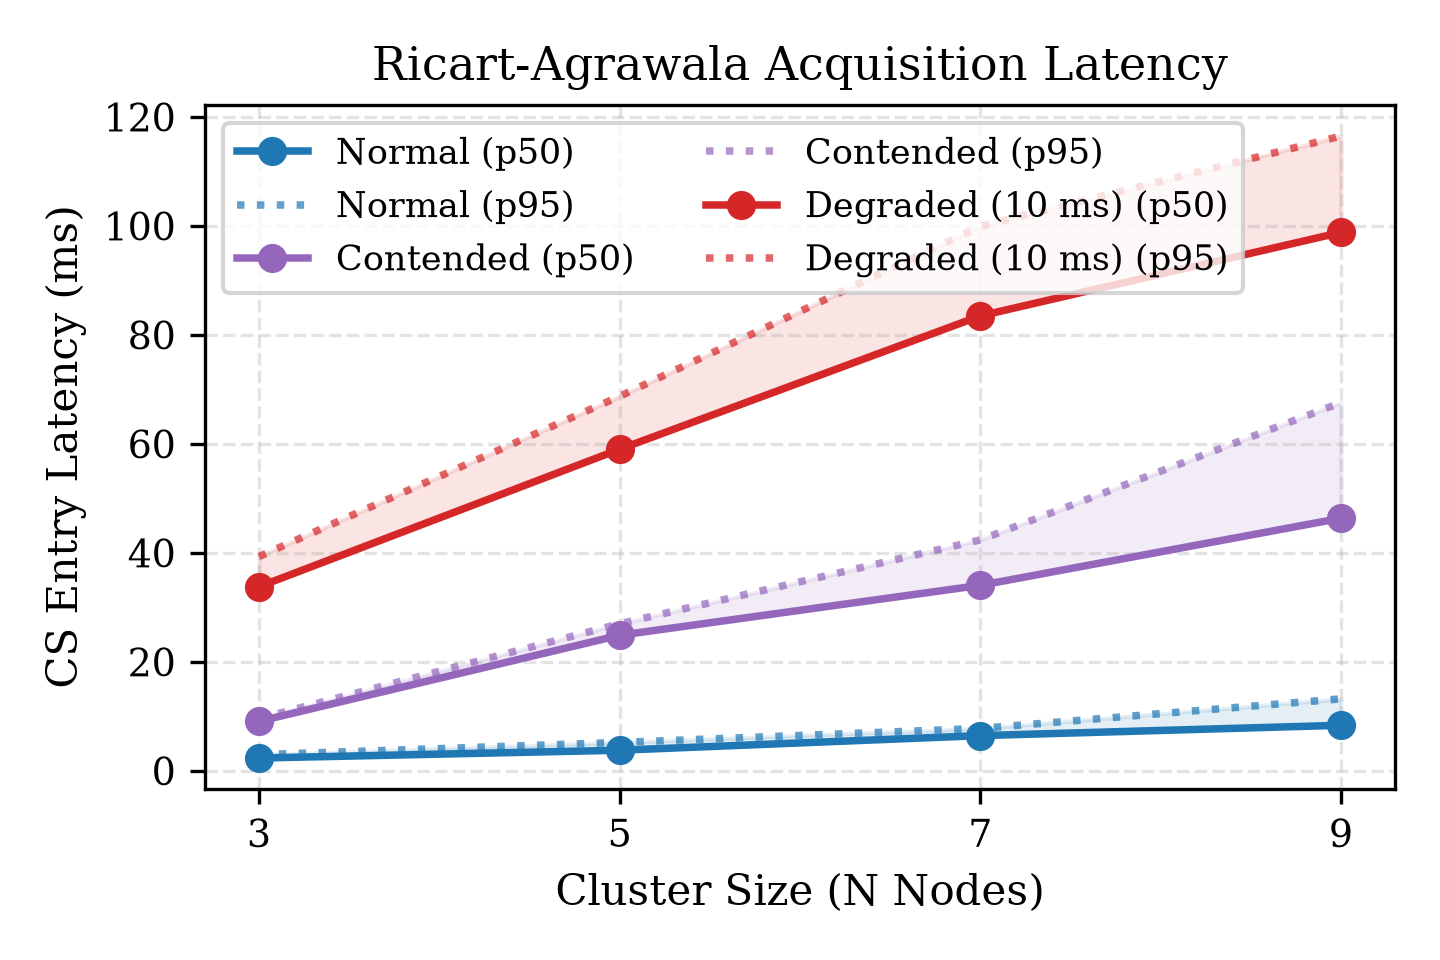
\includegraphics[width=0.92\columnwidth]{exp1_ra_latency.png}
\caption{Latência de entrada na SC (p50 e p95) em função de $N$, nos
cenários normal, com contenção e degradado.}
\label{fig:ra_latency}
\end{figure}

A Tabela~\ref{tab:mensagens} compara a contagem empírica de mensagens com as
fórmulas teóricas. As entradas solo trocaram exatamente $2(N-1)$ mensagens,
ou seja 4, 8, 12 e 16 para os quatro tamanhos de cluster, sem desvio em
nenhuma das repetições, e as entradas sob contenção trocaram exatamente
$N \cdot 2(N-1)$, pois a ordem total não introduz mensagens extras. As
retransmissões não ocorrem sem perdas e são contadas separadamente quando
ocorrem, o que confirma que o mecanismo não interfere no caminho sem falhas
(Figura~\ref{fig:ra_messages}).

\begin{table}[!t]
\centering
\footnotesize
\caption{Mensagens por entrada na SC, medição empírica contra os valores
teóricos $2(N-1)$ (solo) e $N \cdot 2(N-1)$ (contenda).}
\label{tab:mensagens}
\begin{tabular}{ccccc}
\toprule
$N$ & $2(N-1)$ & Solo & $N \cdot 2(N-1)$ & Contenda \\
\midrule
3 & 4  & 4  & 12  & 12  \\
5 & 8  & 8  & 40  & 40  \\
7 & 12 & 12 & 84  & 84  \\
9 & 16 & 16 & 144 & 144 \\
\bottomrule
\end{tabular}
\end{table}

\begin{figure}[!t]
\centering
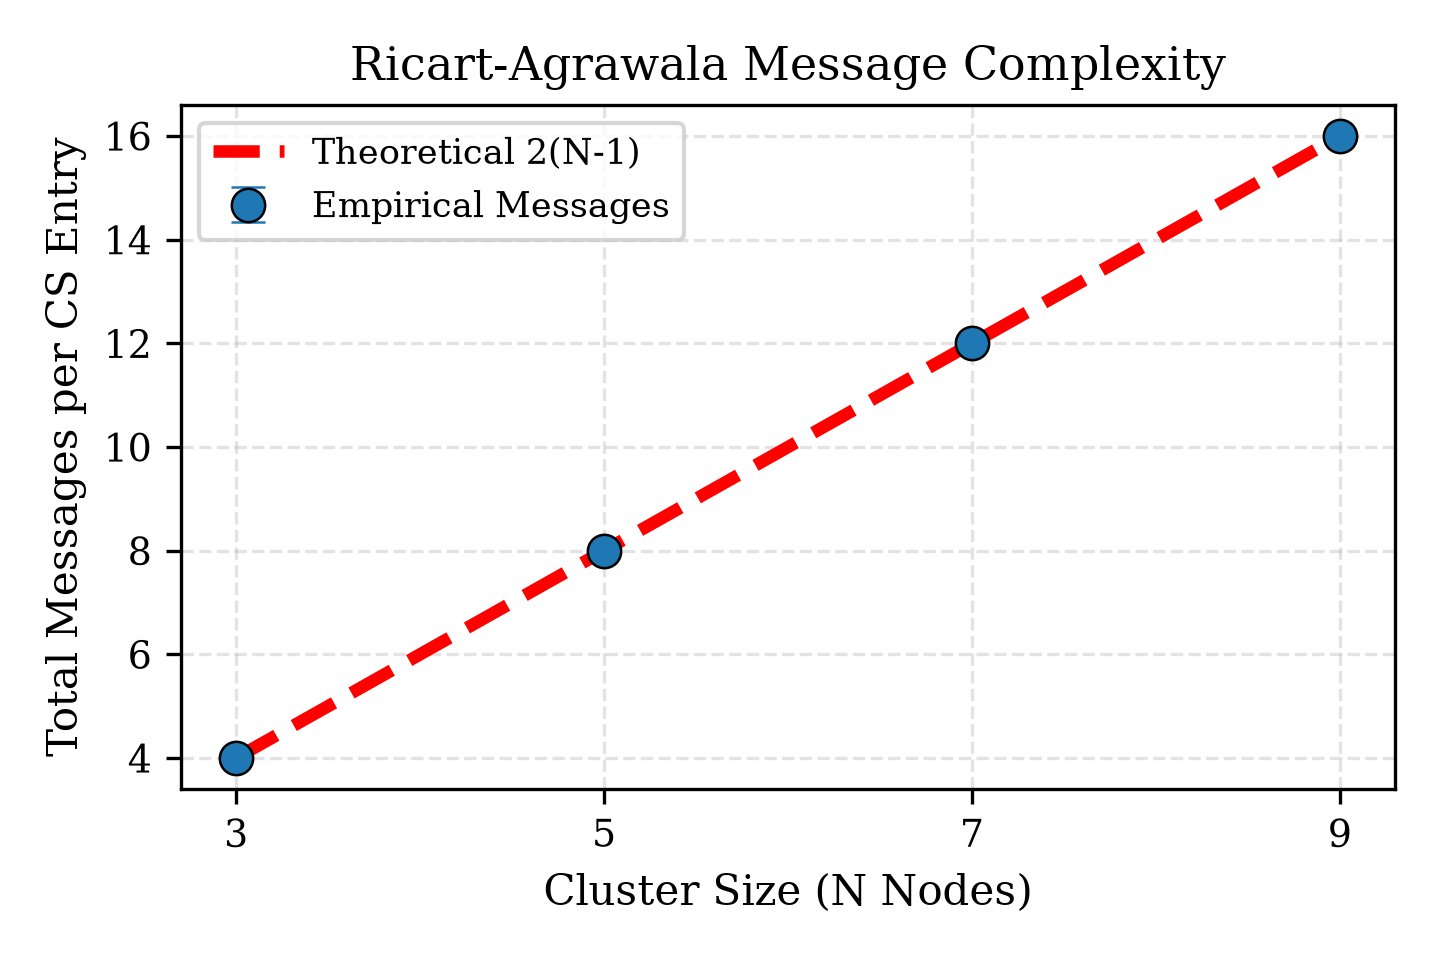
\includegraphics[width=0.92\columnwidth]{exp1_ra_messages.png}
\caption{Mensagens por entrada solo na SC, medição empírica contra a reta
teórica $2(N-1)$.}
\label{fig:ra_messages}
\end{figure}

A latência de commit do 2PC cresce de forma linear com o atraso do canal, com
medianas de 60{,}82 ms, 144{,}87 ms e 243{,}96 ms para $\Delta$ de 5, 25 e
50 ms, como mostram a Tabela~\ref{tab:2pc} e a Figura~\ref{fig:2pc_latency}.
O acréscimo de aproximadamente 4 ms por ms adicional de atraso corresponde às
quatro mensagens do protocolo, PREPARE, voto, decisão e ACK, cada uma
atravessando o canal uma vez, e o termo constante concentra o custo das
gravações persistentes e da conexão por mensagem. As 30 execuções normais
efetivaram com saldos exatos.

\begin{table}[!t]
\centering
\footnotesize
\caption{Experimento 2 com dez repetições por configuração, todas com sucesso
e saldos exatos. Recuperação em média, após queda real do coordenador.}
\label{tab:2pc}
\begin{tabular}{ccccc}
\toprule
$\Delta$ (ms) & p50 commit & p95 commit & Rec. pré-dec. & Rec. pós-dec. \\
\midrule
5  & 60{,}82  & 63{,}85  & 7{,}15 & 6{,}10 \\
25 & 144{,}87 & 146{,}80 & 8{,}54 & 6{,}72 \\
50 & 243{,}96 & 249{,}82 & 7{,}98 & 6{,}97 \\
\bottomrule
\end{tabular}
\end{table}

\begin{figure}[!t]
\centering
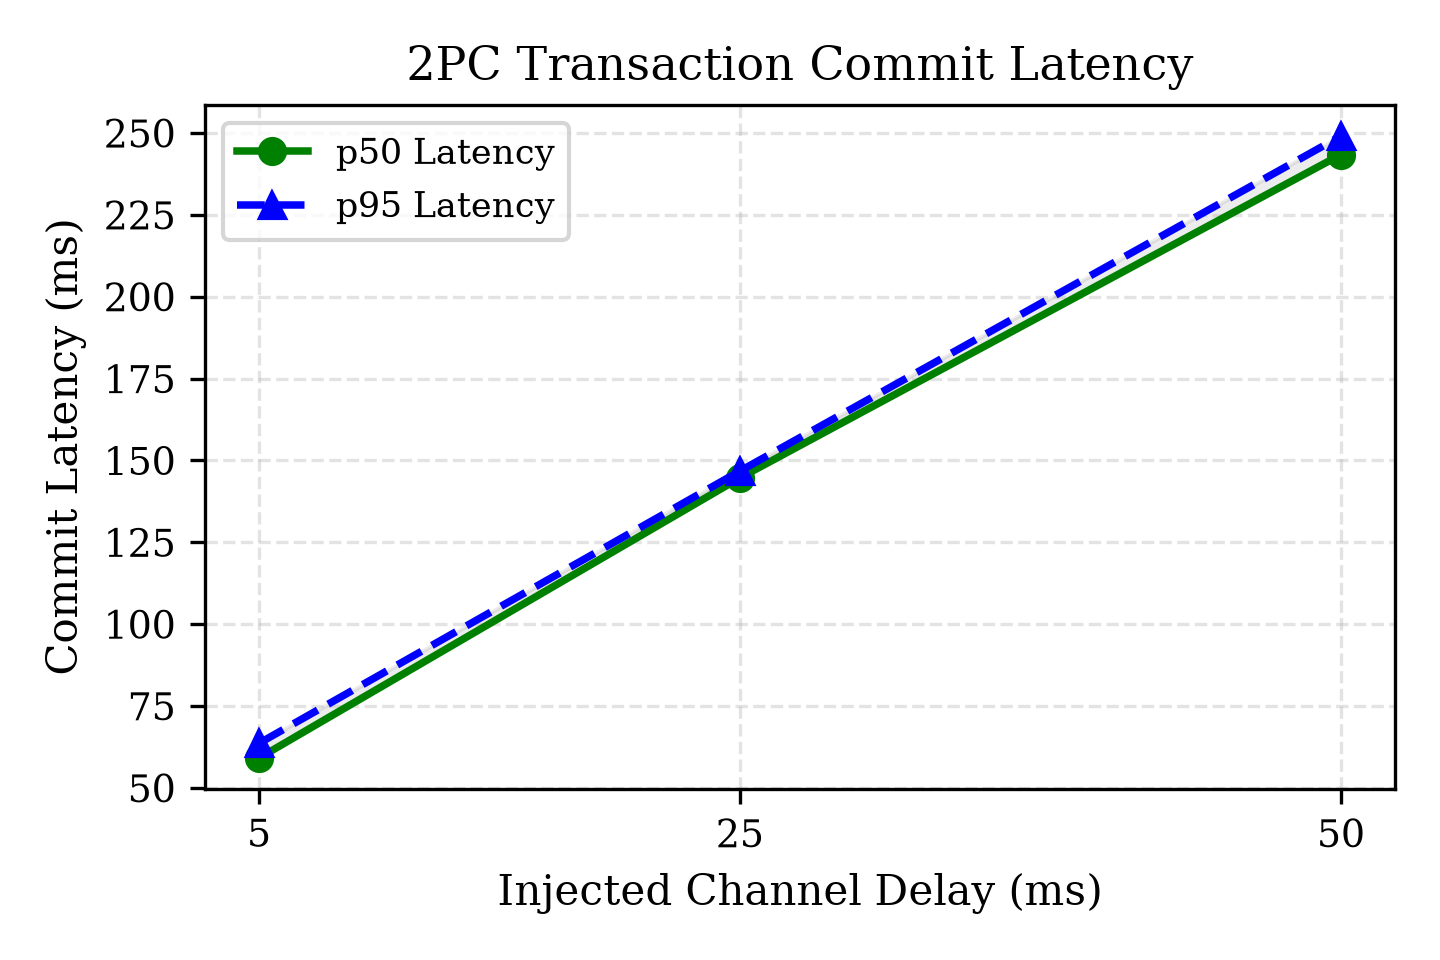
\includegraphics[width=0.92\columnwidth]{exp2_2pc_latency.png}
\caption{Latência de commit do 2PC (p50 e p95) sob diferentes atrasos de
canal injetados.}
\label{fig:2pc_latency}
\end{figure}

Nos cenários de queda real do coordenador, as 60 execuções convergiram ao
desfecho correto com saldos exatos em todas. A queda antes da decisão resulta
em \emph{Presumed Abort} com saldos intactos, e a queda após o registro de
\texttt{COMMITTED} resulta em redecisão com repropagação e ambos os nós
aplicando as operações. A recuperação completa, com reprodução do WAL,
reconstrução do saldo e resolução das transações, leva de 6 a 9 ms na média e
não cresce com o atraso injetado, pois é dominada pela leitura sequencial do
log e pela reaplicação local (Figura~\ref{fig:2pc_recovery}).

\begin{figure}[!t]
\centering
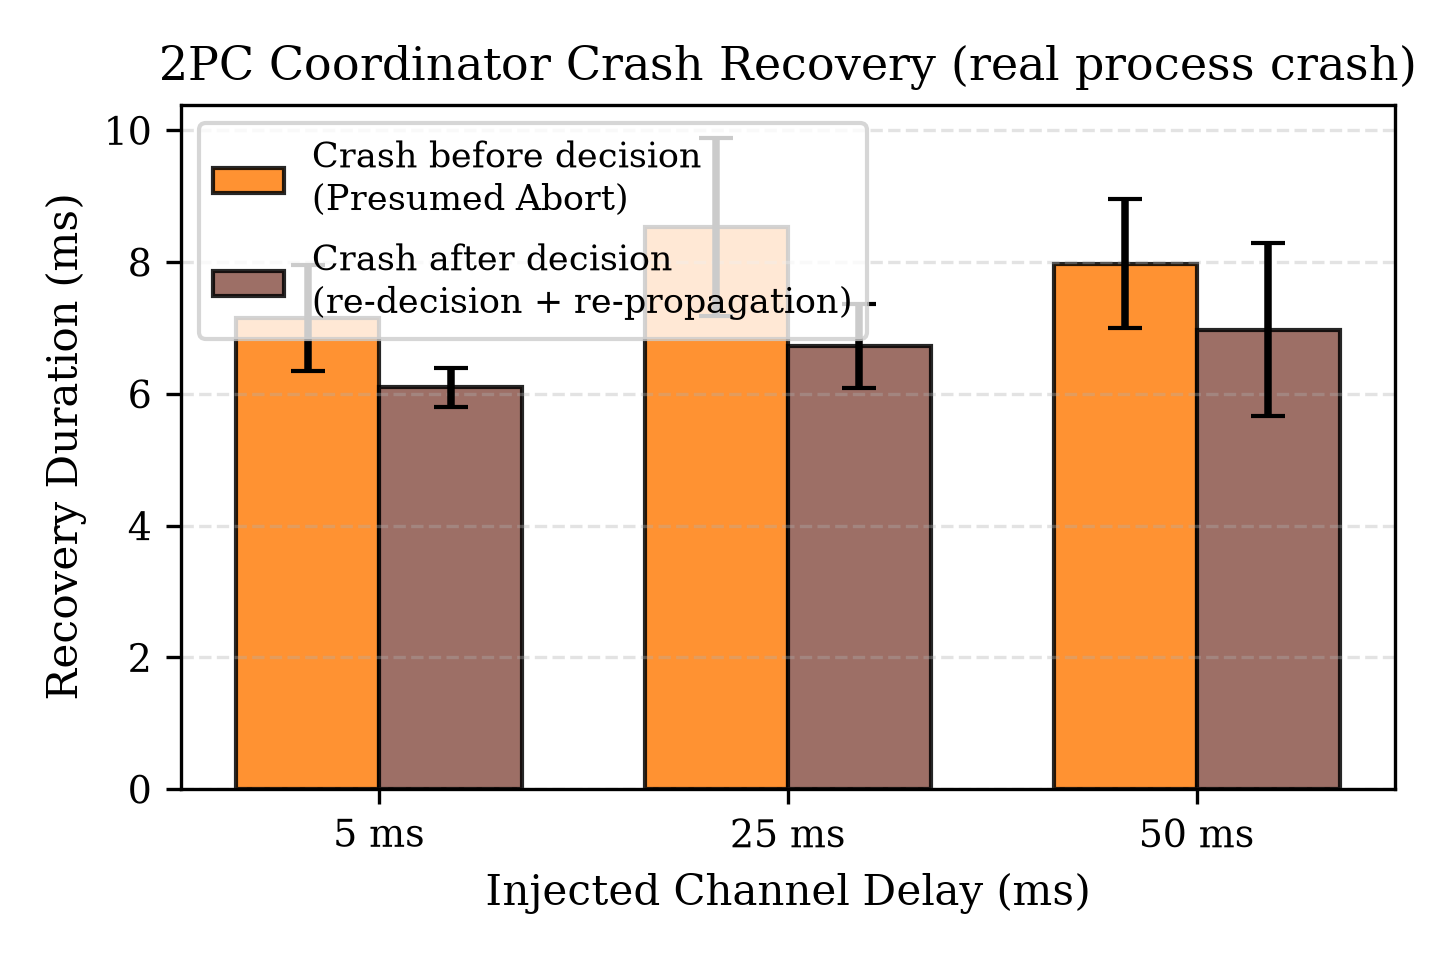
\includegraphics[width=0.92\columnwidth]{exp2_2pc_recovery.png}
\caption{Tempo de recuperação após queda real do processo coordenador, por
ponto de falha e atraso de canal.}
\label{fig:2pc_recovery}
\end{figure}

O tempo de convergência do snapshot permanece estável com a carga em rede
desimpedida, com medianas entre 6{,}50 ms e 7{,}29 ms para todas as taxas, e
cresce com o atraso dos marcadores sob \emph{jitter}, de 28{,}90 ms a
38{,}81 ms, como mostram a Tabela~\ref{tab:snap} e a
Figura~\ref{fig:snapshot_duration}. Esse comportamento é compatível com a
complexidade $O(N)$ de mensagens do algoritmo, independente do tráfego. Em
todas as 60 execuções com tráfego concorrente a auditoria registrou
exatamente 3000{,}00, incluindo execuções com transferências capturadas em
trânsito nos canais, o que valida a captura de cortes consistentes e o
portão de ordenação entre marcadores e mensagens de aplicação
(Figura~\ref{fig:snapshot_conservation}).

\begin{table}[!t]
\centering
\footnotesize
\caption{Experimento 3, duração do snapshot em ms por taxa de
transferências, com conservação patrimonial em 60 de 60 execuções.}
\label{tab:snap}
\begin{tabular}{ccccc}
\toprule
$\lambda$ (tx/s) & p50 calmo & p95 calmo & p50 jitter & p95 jitter \\
\midrule
10 & 7{,}19 & 8{,}14 & 33{,}12 & 38{,}36 \\
25 & 6{,}50 & 8{,}35 & 28{,}90 & 39{,}27 \\
50 & 7{,}29 & 8{,}61 & 38{,}81 & 46{,}09 \\
\bottomrule
\end{tabular}
\end{table}

\begin{figure}[!t]
\centering
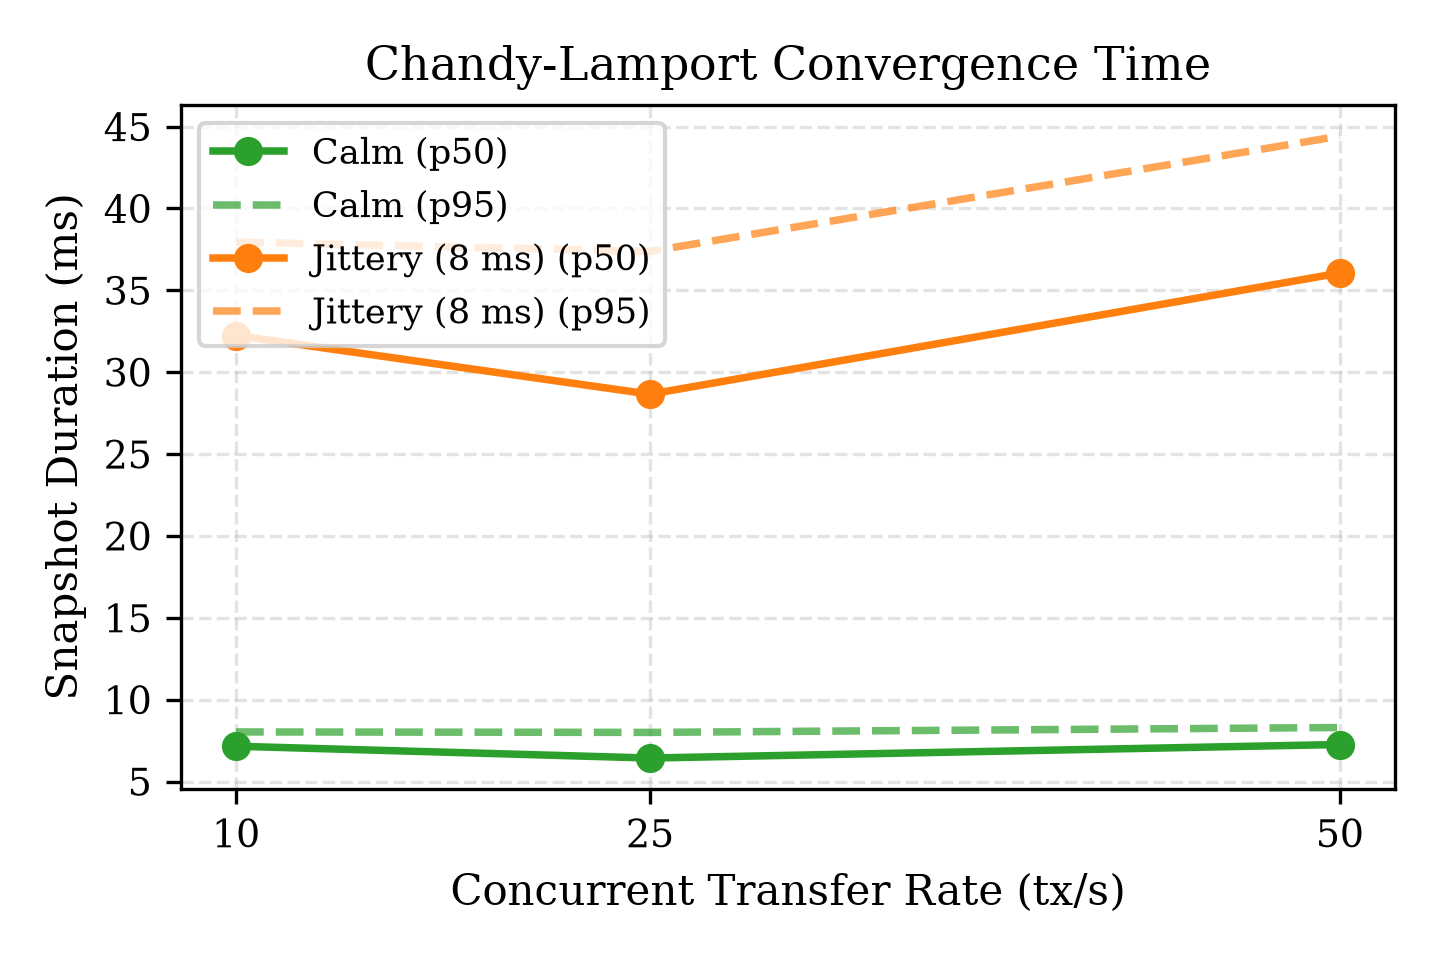
\includegraphics[width=0.92\columnwidth]{exp3_snapshot_duration.png}
\caption{Tempo de convergência do snapshot de Chandy-Lamport (p50 e p95)
para diferentes taxas de transferências concorrentes.}
\label{fig:snapshot_duration}
\end{figure}

\begin{figure}[!t]
\centering
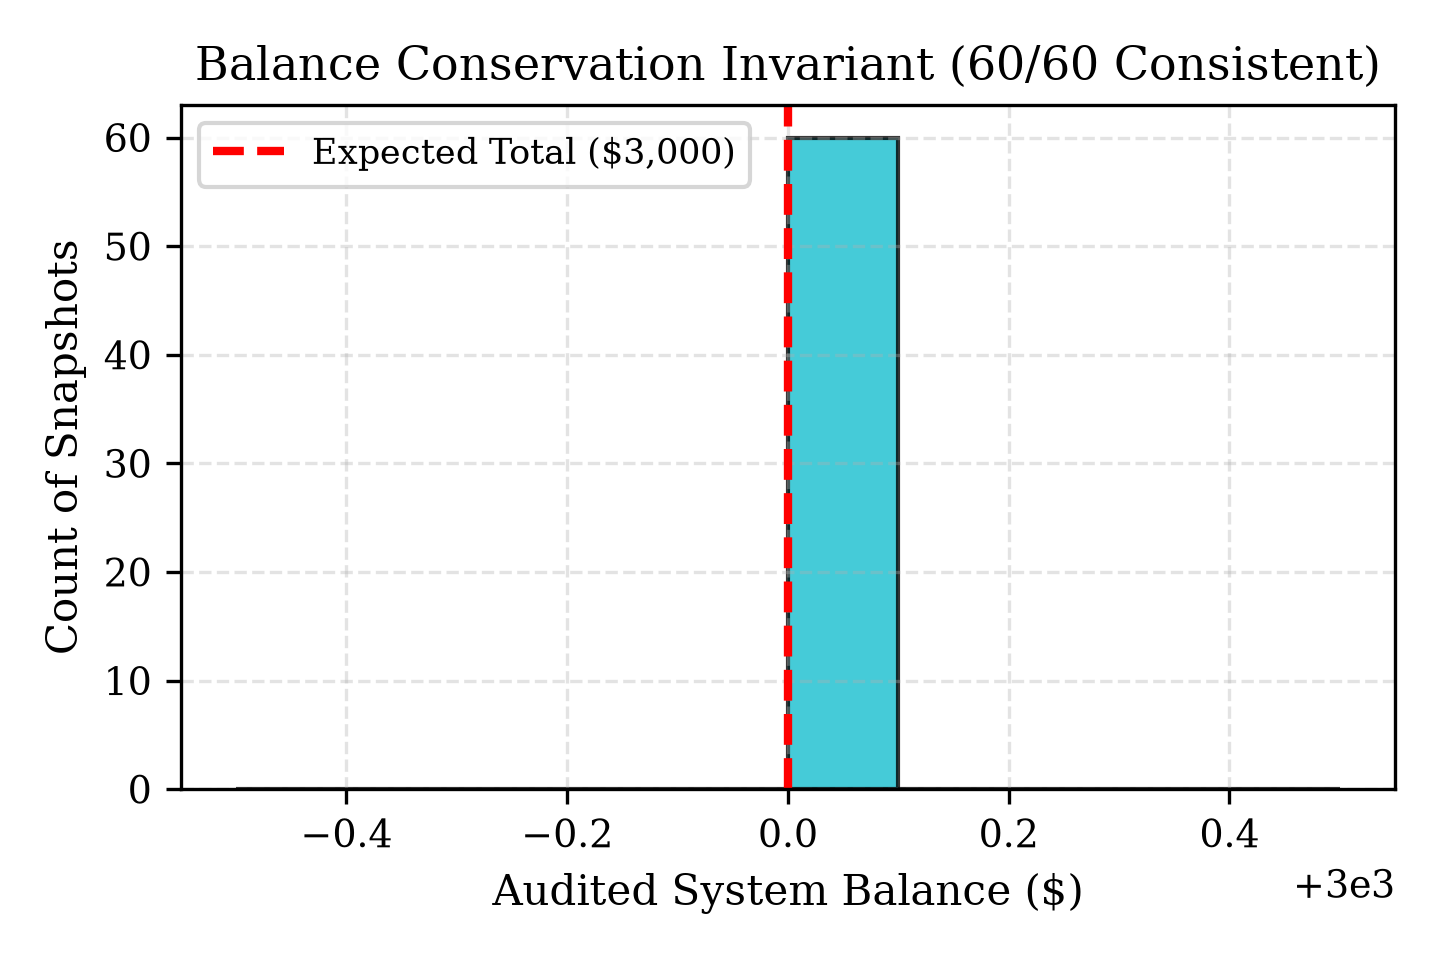
\includegraphics[width=0.92\columnwidth]{exp3_snapshot_conservation.png}
\caption{Saldo patrimonial auditado em todos os ensaios de snapshot, com
conservação em 100\% das execuções.}
\label{fig:snapshot_conservation}
\end{figure}

\begin{itemize}
    \item \textbf{Consistência global:} os 270 ensaios das três campanhas
    produziram desfechos corretos em 100\% das execuções dos experimentos 2 e
    3, com saldos finais exatos em todos os cenários, incluindo os de queda
    real do processo coordenador.
    \item \textbf{Independência da recuperação:} o tempo de recuperação não
    varia com o atraso do canal, pois o processo reiniciado recomeça com
    configuração de falhas limpa e o custo é dominado pela reprodução do WAL,
    e não pela rede.
    \item \textbf{Comportamento dos percentis:} a distância entre p50 e p95
    cresce com a contenção e com o \emph{jitter}, refletindo a variabilidade
    da ordem de Lamport sob disputa e do atraso amostrado nos canais.
    \item \textbf{Ausência de mensagens extras:} a contagem exata em todos os
    cenários confirma que nem a retransmissão idempotente nem a integração
    com o 2PC alteram a complexidade de mensagens do algoritmo.
\end{itemize}

\section{Divisão de Trabalho}
\begin{itemize}
    \item \textbf{Celso Gabriel Prado:} módulos \texttt{network} (canal TCP,
    protocolo de mensagens e injetor de falhas) e \texttt{mutual\_exclusion}
    (relógio de Lamport e Ricart-Agrawala com retransmissão), a suíte de
    testes automatizados, os scripts e os dados dos experimentos, e parte
    deste relatório.
    \item \textbf{Giovanni Santos Scalabrin:} módulos \texttt{atomic\_commit}
    (WAL, 2PC e recuperação) e \texttt{snapshot} (Chandy-Lamport e auditor),
    os módulos \texttt{node} e \texttt{cli} (integração da aplicação e plano
    de controle), e parte deste relatório.
\end{itemize}

\section*{Código e Instruções de Execução}
O código-fonte (Python 3, sem dependências para a lógica distribuída)
acompanha esta entrega no repositório, com as instruções completas de
instalação e execução no arquivo \texttt{README.md}. Em resumo, \texttt{make
test} executa a suíte de 23 testes, \texttt{make bench} roda as três campanhas
de experimentos com nós em processos independentes, \texttt{make plots} gera
as figuras a partir dos dados brutos e \texttt{make report} compila este
documento. O cluster de cinco nós em contêineres sobe com \texttt{docker
compose up}, e os comandos do cliente, como \texttt{python3 -m
distrib\_ledger.cli client transfer -{}-to node2 -{}-amount 150}, operam o
sistema em execução, incluindo injeção de falhas e auditoria de snapshots.

\section*{Nota sobre Uso de Ferramentas de IA}
Durante o desenvolvimento deste trabalho, a dupla utilizou ferramentas de IA
generativa como apoio na escrita da estrutura inicial do projeto (esqueleto
dos módulos, da interface de linha de comando e da organização do
repositório). Todo o resto do código, o modelo do sistema apresentado, a
análise dos experimentos e a redação deste relatório são de autoria da dupla,
salvo uso de LLMs para correção ortográfica.

\section{Conclusão}
Neste trabalho foram implementados e avaliados três algoritmos distribuídos
integrados em uma aplicação coerente de liquidação financeira, com exclusão
mútua por Ricart-Agrawala, compromisso atômico por 2PC com WAL e
observabilidade global por Chandy-Lamport, executados sobre nós independentes
que se comunicam exclusivamente pela rede.

Os resultados confirmaram as propriedades esperadas de cada algoritmo. A
contagem de mensagens coincidiu com $2(N-1)$ em todas as entradas solo e com
$N \cdot 2(N-1)$ sob contenção, a latência de entrada cresceu linearmente com
o número de nós, a latência de commit acompanhou o atraso do canal com
inclinação compatível com as quatro mensagens do protocolo, e a recuperação
de quedas reais do coordenador concluiu em 6 a 9 ms com o desfecho correto em
todas as 60 execuções. A conservação patrimonial foi verificada em 60 de 60
snapshots sob tráfego concorrente, com total exato de 3000{,}00.

Do ponto de vista prático, os compromissos declarados permanecem. A
retransmissão preserva a segurança da exclusão mútua sob perdas de mensagens,
ao custo de bloquear novas entradas quando um par cai permanentemente, e o
2PC mantém participantes in-doubt bloqueados até que a consulta cooperativa
resolva, limitação que protocolos de maioria como Raft e Paxos eliminam ao
custo de mais mensagens. De modo geral, a integração dos três algoritmos em
uma única aplicação mostrou que serialização, atomicidade e observação global
podem coexistir sobre canais TCP comuns, com propriedades verificáveis por
testes automatizados e experimentos reproduzíveis.

\begin{thebibliography}{9}

\bibitem{vansteen2023}
M. van Steen e A. S. Tanenbaum, \emph{Distributed Systems}, 4th ed. distributed-systems.net, 2023.

\bibitem{lamport1978time}
L. Lamport, ``Time, clocks, and the ordering of events in a distributed system,'' \emph{Communications of the ACM}, vol. 21, no. 7, pp. 558-565, 1978.

\bibitem{ricart1981algorithm}
G. Ricart e A. K. Agrawala, ``An optimal algorithm for mutual exclusion in computer networks,'' \emph{Communications of the ACM}, vol. 24, no. 1, pp. 9-17, 1981.

\bibitem{chandy1985distributed}
K. M. Chandy e L. Lamport, ``Distributed snapshots: Determining global states of distributed systems,'' \emph{ACM Transactions on Computer Systems (TOCS)}, vol. 3, no. 1, pp. 63-75, 1985.

\bibitem{gray1978notes}
J. Gray, ``Notes on data base operating systems,'' in \emph{Operating Systems, An Advanced Course}, Lecture Notes in Computer Science, vol. 60. Springer, 1978, pp. 393-481.

\bibitem{fischer1985impossibility}
M. J. Fischer, N. A. Lynch, e M. S. Paterson, ``Impossibility of distributed consensus with one faulty process,'' \emph{Journal of the ACM (JACM)}, vol. 32, no. 2, pp. 374-382, 1985.

\end{thebibliography}

\end{document}
